\documentclass[12pt]{IEEEtran}
\usepackage{amsthm}
\usepackage{url}
\usepackage{graphicx}

\begin{document}

\title{\bf CSP203 Project Proposal \\
            Android Smart City Traveler}

\author{

Prasad Kshirsagar\\
2016CSB1041

}


\maketitle
\textbf{ Abstract - In this Proposal, I have presented my view to develop this application. It also includes features, advantages, appliations of the app.}\\ \hfill \break 
 

\textbf{
Index Terms - Android, Traveler,City
}


 \section{Introduction :}
  The purpose of developing this android application is to create a schedule for the traveler travelling to city and wanted to explore the city by specifying the time in hours. System then smartly analyzes the questionnaire and creates a schedule for traveler based on provided time.\\ \hfill \break 
  
  
 \section{How to Proceed :}
  The development will be done in two technical languages as Java for Android Application for User/Traveler and Asp .net for Web portal which is used by Admin.First of all, traveler need to register himself by filling up the details using android application. After successful registration, user can login now using login credentials which then proceeds with questionnaire where application ask user about their likings and habits. Based on questionnaire, application smartly analyzes for the place based on user specified time.\\ 

\section{Objectives :}
   \begin{itemize}
  \item The application will be capable enough to search the place automatically based on FourSquare API.
  \item This application will also help you to find the places nearby you or around the world.
  \item After searching a place, the map will show the details such as name, area, location, phone no, kilometers from the current location of the user.
  \end{itemize} \hfill \break
  

\begin{figure}
\centering
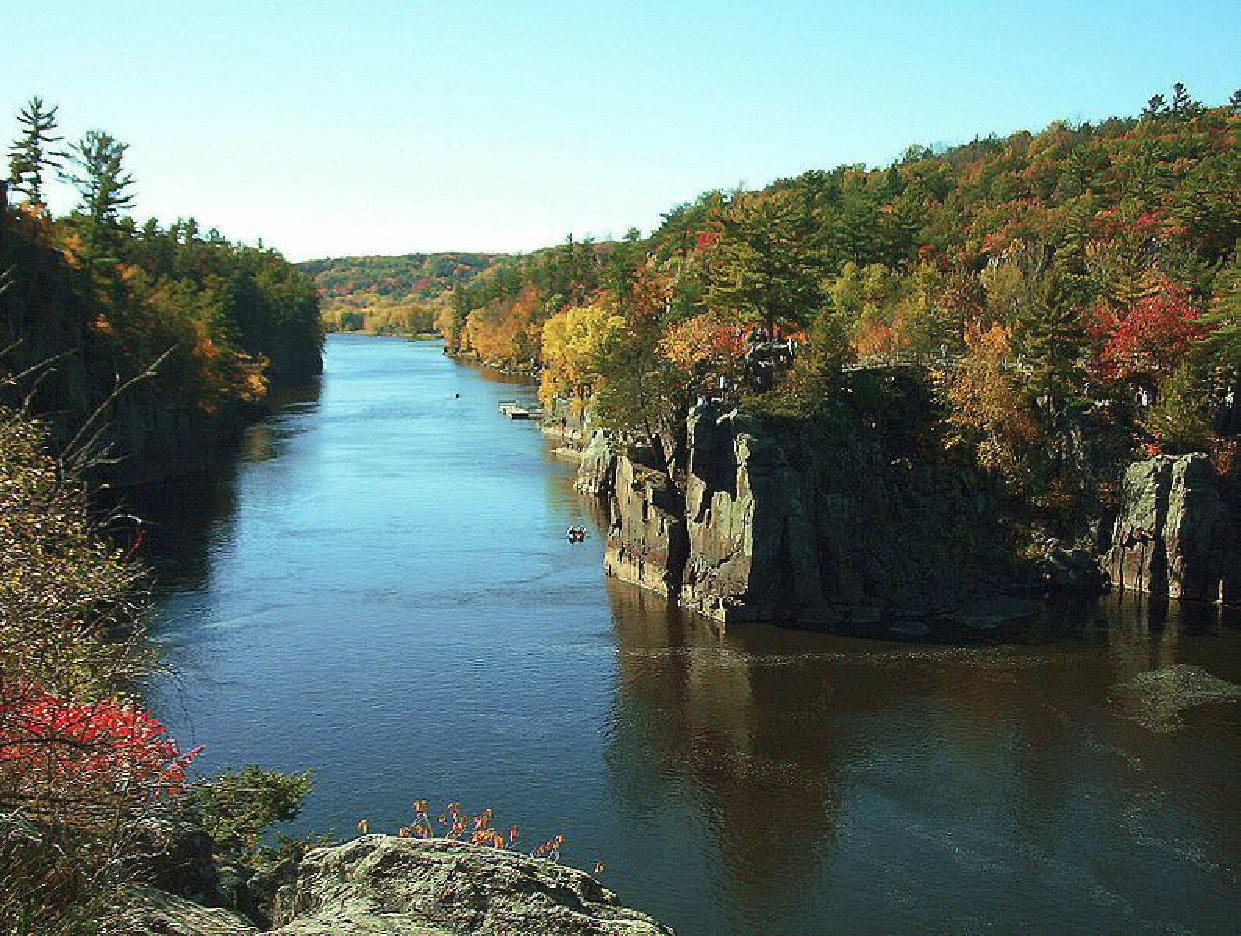
\includegraphics[width=1\linewidth]{111.pdf}
\label{fig:block-diagram}
\end{figure}
%Adding * spans the figure over two columns.

\section{Features :}
   \begin{itemize}
   \item Login page which allows only the registered user to login and thereby preventing unauthorized access.
   \item Can view the location view in map that the user wishes to reach.
   \item Proper time management.
   \end{itemize} \hfill \break

\section{Advantages :}
  \begin{itemize}
  \item The user can also find the paths to follow to reach the final destination in map which gives a better view to the users.
  \item Since the location can be viewed in map, the user can even zoom in and zoom out to get a better view.
  \item The usage of this application greatly reduces the time required to search for a place.
  \item The application also leads to quicker decision making with respect to places to visit.
  \end{itemize} \hfill \break


\section{Applications :}
  \subsection{Tourism industry :}
  This application will be helpful in this industry because of its power to track various stations in limited time.
  \subsection{Personal use :}
  We can use our time better by taking help of this app.
  
  
  

\bibliographystyle{abbrv}
\bibliography{reference} 
\end{document}
